\documentclass[12pt]{report}
\usepackage[utf8]{inputenc}
\usepackage[russian]{babel}
%\usepackage[14pt]{extsizes}
\usepackage{listings}
\usepackage{graphicx}
\usepackage{amsmath,amsfonts,amssymb,amsthm,mathtools} 

% Для листинга кода:
\lstset{ %
language=python,                 % выбор языка для подсветки (здесь это С)
basicstyle=\small\sffamily, % размер и начертание шрифта для подсветки кода
numbers=left,               % где поставить нумерацию строк (слева\справа)
numberstyle=\tiny,           % размер шрифта для номеров строк
stepnumber=1,                   % размер шага между двумя номерами строк
numbersep=5pt,                % как далеко отстоят номера строк от подсвечиваемого кода
showspaces=false,            % показывать или нет пробелы специальными отступами
showstringspaces=false,      % показывать или нет пробелы в строках
showtabs=false,             % показывать или нет табуляцию в строках
frame=single,              % рисовать рамку вокруг кода
tabsize=2,                 % размер табуляции по умолчанию равен 2 пробелам
captionpos=t,              % позиция заголовка вверху [t] или внизу [b] 
breaklines=true,           % автоматически переносить строки (да\нет)
breakatwhitespace=false, % переносить строки только если есть пробел
escapeinside={\#*}{*)}   % если нужно добавить комментарии в коде
}

% Для измененных титулов глав:
\usepackage{titlesec, blindtext, color} % подключаем нужные пакеты
\definecolor{gray75}{gray}{0.75} % определяем цвет
\newcommand{\hsp}{\hspace{20pt}} % длина линии в 20pt
% titleformat определяет стиль
\titleformat{\chapter}[hang]{\Huge\bfseries}{\thechapter\hsp\textcolor{gray75}{|}\hsp}{0pt}{\Huge\bfseries}


% plot
\usepackage{pgfplots}
\usepackage{filecontents}
\usetikzlibrary{datavisualization}
\usetikzlibrary{datavisualization.formats.functions}
\begin{filecontents}{LevR.dat}
1 5928
2 16865
3 62333
4 372661
5 1909255
6 9065189
7 45325069
\end{filecontents}

\begin{filecontents}{LevT.dat}
1 3724258
2 7224736
3 12123365
4 16940041
5 23402008
6 32328258
7 30166031
\end{filecontents}

\begin{filecontents}{DamLevR.dat}
1 7456
2 21845
3 105445
4 407763
5 1966658
6 11002094
7 51219656
\end{filecontents}

\begin{filecontents}{DamLevT.dat}
1 4367560
2 8286833
3 12852145
4 18585284
5 24103230
6 27935583
7 30567571
\end{filecontents}


\begin{document}
%\def\chaptername{} % убирает "Глава"
\begin{titlepage}
	\centering
	{\scshape\LARGE МГТУ им. Баумана \par}
	\vspace{3cm}
	{\scshape\Large Лабораторная работа №1\par}
	\vspace{0.5cm}	
	{\scshape\Large По курсу: "Анализ алгоритмов"\par}
	\vspace{1.5cm}
	{\huge\bfseries Расстояние Левенштейна\par}
	\vspace{2cm}
	\Large Работу выполнила: Лаврова Анастасия, ИУ7-55Б\par
	\vspace{0.5cm}
	\LargeПреподаватели:  Волкова Л.Л., Строганов Ю.В.\par

	\vfill
	\large \textit {Москва, 2019} \par
\end{titlepage}

\tableofcontents

\newpage
\chapter*{Введение}
\addcontentsline{toc}{chapter}{Введение}
\textbf{Расстояние Левенштейна} - минимальное количество операций вставки одного символа, удаления одного символа и замены одного символа на другой, необходимых для превращения одной строки в другую.

Расстояние Левенштейна применяется в теории информации и компьютерной лингвистике для:

\begin{itemize}
	\item исправления ошибок в слове
	\item сравнения текстовых файлов утилитой diff
	\item в биоинформатике для сравнения генов, хромосом и белков
\end{itemize}

Целью данной лабораторной работы является изучение метода динамического программирования на материале алгоритмов
Левенштейна и Дамерау-Левенштейна. 

Задачами данной лабораторной являются:
\begin{enumerate}
  	\item изучение алгоритмов Левенштейна и Дамерау-Левенштейна нахождения расстояния между строками;
	\item применение метода динамического программирования для матричной реализации указанных алгоритмов; 
	\item получение практических навыков реализации указанных алгоритмов: двух алгоритмов в матричной версии и одного из алгоритмов в рекурсивной версии; 
	\item сравнительный анализ линейной и рекурсивной реализаций выбранного алгоритма определения расстояния между строками по затрачиваемым ресурсам (времени и памяти); 
	\item экспериментальное подтверждение различий во временнóй эффективности рекурсивной и
нерекурсивной реализаций выбранного алгоритма определения расстояния между строками при
помощи разработанного программного обеспечения на материале замеров процессорного времени
выполнения реализации на варьирующихся длинах строк; 
	\item описание и обоснование полученных результатов в отчете о выполненной лабораторной
работе, выполненного как расчётно-пояснительная записка к работе. 
\end{enumerate}


\chapter{Аналитическая часть}
Задача по нахождению расстояния Левенштейна заключается в поиске минимального количества операций вставки/удаления/замены для превращения одной строки в другую.

При нахождении расстояния Дамерау — Левенштейна добавляется операция транспозиции (перестановки соседних символов).  
 
\textbf{Действия обозначаются так:} 
\begin{enumerate}
  	\item D (англ. delete) — удалить,
	\item I (англ. insert) — вставить,
	\item R (replace) — заменить,
	\item M(match) - совпадение.
\end{enumerate}

Пусть $S_{1}$ и $S_{2}$ — две строки (длиной M и N соответственно) над некоторым алфавитом, тогда расстояние Левенштейна можно подсчитать по следующей рекуррентной формуле:

\begin{displaymath}
D(i,j) = \left\{ \begin{array}{ll}
 0, & \textrm{$i = 0, j = 0$}\\
 i, & \textrm{$j = 0, i > 0$}\\
 j, & \textrm{$i = 0, j > 0$}\\
min(\\
D(i,j-1)+1,\\
D(i-1, j) +1, &\textrm{$j>0, i>0$}\\
D(i-1, j-1) + m(S_{1}[i], S_{2}[j])\\
),
  \end{array} \right.
\end{displaymath}

где $m(a,b)$ равна нулю, если $a=b$ и единице в противном случае; $min\{\,a,b,c\}$ возвращает наименьший из аргументов.

Расстояние Дамерау-Левенштейна вычисляется по следующей рекуррентной формуле:
		    
		     \[ D(i, j) =  \left\{
			\begin{aligned}
				&0, && i = 0, j = 0\\
		    	&i, && i > 0, j = 0\\
		    	&j, && i = 0, j > 0\\		    	
		    	&min \left\{
				\begin{aligned}
					&D(i, j - 1) + 1,\\
		            &D(i - 1, j) + 1,\\
		            &D(i - 1, j - 1) + m(S_{1}[i], S_{2}[i]), \\
		            &D(i - 2, j - 2) + m(S_{1}[i], S_{2}[i]),\\
		        \end{aligned} \right.
		        && 
				\begin{aligned}
					&, \text{ если } i, j > 0 \\
		            & \text{ и } S_{1}[i] = S_{2}[j - 1] \\
		            & \text{ и } S_{1}[i - 1] =  S_{2}[j] \\
		        \end{aligned} \\ 
		        &min \left\{
		        \begin{aligned}
		            &D(i, j - 1) + 1,\\
		            &D(i - 1, j) + 1, \\
		            &D(i - 1, j - 1) + m(S_{1}[i], S_{2}[i]),\\
		        \end{aligned} \right.  &&, \text{иначе}
			\end{aligned} \right.
			\]	
	    
		\subsection{Вывод}
		В данном разделе были рассмотрены алгоритмы нахождения расстояния Левенштейна и Дамерау-Левенштейна, который является модификаций первого, учитывающего возможность перестановки соседних символов. 




\chapter{Конструкторская часть}
\textbf{Требования к вводу:}
\begin{enumerate}
  	\item На вход подаются две строки
	\item uppercase и lowercase буквы считаются разными
\end{enumerate}
\textbf{Требования к программе:}
\begin{enumerate}
  	\item Две пустые строки - корректный ввод, программа не должна аварийно завершаться
\end{enumerate}
\section{Схемы алгоритмов}
В данной части будут рассмотрены схемы алгоритмов.

\begin{figure}[h]
\centering
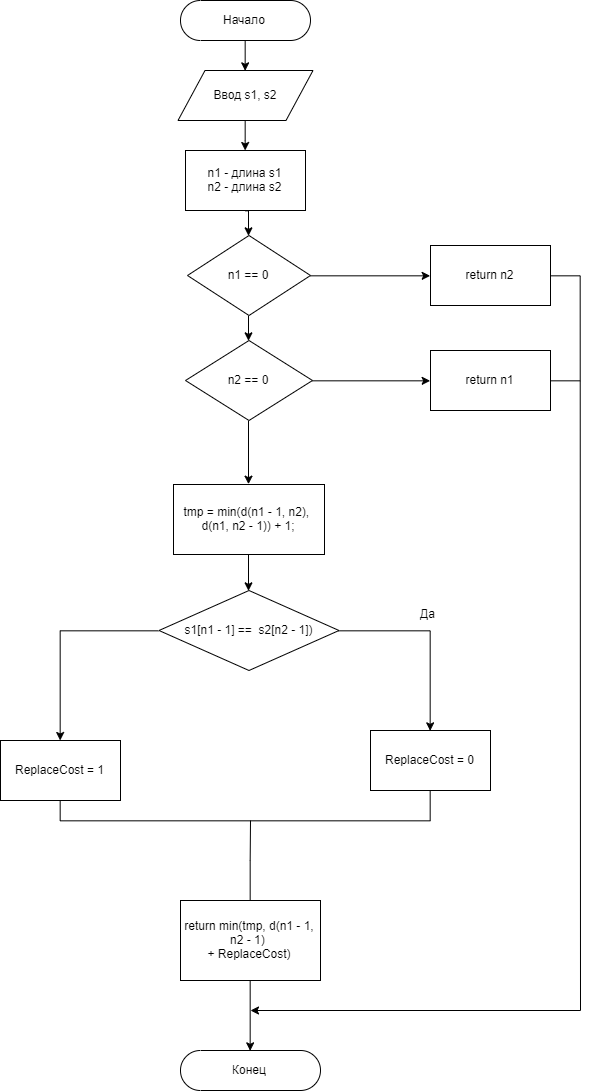
\includegraphics[width=0.75\linewidth]{RecLev.png}
\caption{Схема рекурсивного алгоритма нахождения расстояния Левенштейна}
\label{fig:mpr}
\end{figure}


\begin{figure}[h]
\centering
\includegraphics[width=0.6\linewidth]{MatrixL.jpg}
\caption{Схема матричного алгоритма нахождения расстояния Левенштейна}
\label{fig:mpr}
\end{figure}


\begin{figure}[h]
\centering
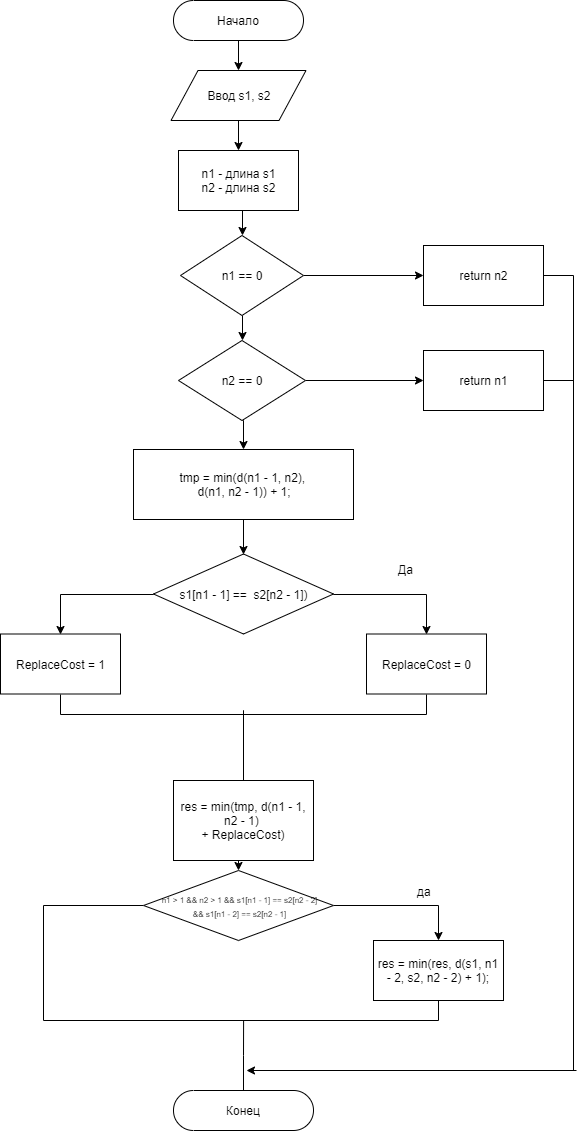
\includegraphics[width=0.75\linewidth]{RecDL.png}
\caption{Схема рекурсивного алгоритма нахождения расстояния Дамерау-Левенштейна}
\label{fig:mpr}
\end{figure}

\begin{figure}[h]
\centering
\includegraphics[width=0.75\linewidth]{MatrixDL.jpg}
\caption{Схема матричного алгоритма нахождения расстояния Дамерау-Левенштейна}
\label{fig:mpr}
\end{figure}


\chapter{Технологическая часть}
\section{Выбор ЯП}
Для реализации программ я выбрала язык программирования C++, так имею большой опыт работы с ним. Среда разработки - Visual Studio.

\begin{figure}[h]
\centering
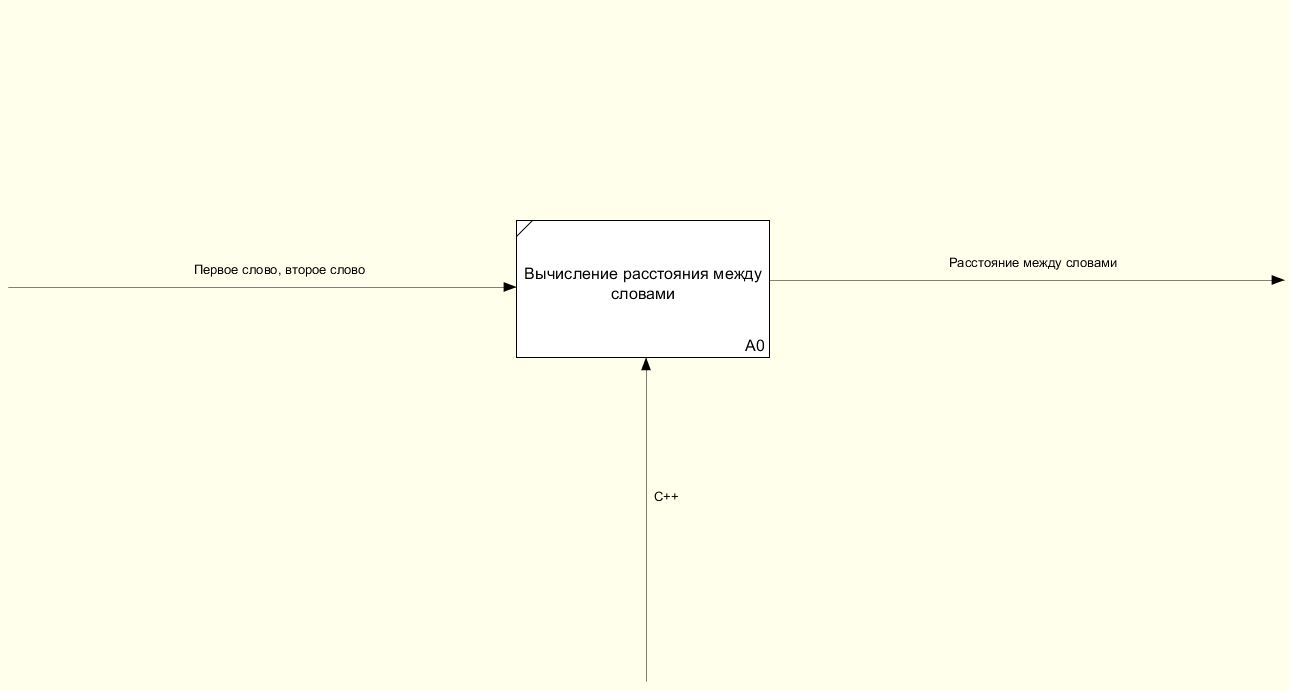
\includegraphics[width=1\linewidth]{idef.jpg}
\caption{IDEF0-диаграмма, описывающая алгоритм нахождения расстояния Левенштейна}
\label{fig:mpr}
\end{figure}


\section{Реализация алгоритма}

\begin{lstlisting}[label=some-code,caption=Функция нахождения расстояния Левенштейна рекурсивно]
int levenshtein_rec(string &s1, int n1, string &s2, int n2)
{
	if (n1 == 0)
		return n2;
	if (n2 == 0)
		return n1;
	unsigned int tmp = min(levenshtein_rec(s1, n1 - 1, s2, n2), 
		levenshtein_rec(s1, n1, s2, n2 - 1)) + 1;
	return min(tmp, levenshtein_rec(s1, n1 - 1, s2, n2 - 1) 
		+ ReplaceCost(s1[n1 - 1], s2[n2 - 1]));
}
\end{lstlisting}

\begin{lstlisting}[label=some-code,caption=Функция нахождения штрафа]
unsigned int ReplaceCost(char a, char b)
{
	return (a != b);
}
\end{lstlisting}

\begin{lstlisting}[label=some-code,caption=Функция нахождения расстояния Левенштейна матрично]
int levenshtein_matrix(string s1, string s2)
{
	int len_s1 = s1.length();
	int len_s2 = s2.length();
	if (len_s1 == 0)
		return len_s2;
	if (len_s2 == 0)
		return len_s1;

	int **matrix = (int**)malloc((len_s1+1) * sizeof(int*));
	for (int i = 0; i <= len_s1; i++)
	{
		matrix[i] = (int*)malloc((len_s2 + 1) * sizeof(int));
	}

	for (int i = 0; i <= len_s1; i++)
	{
		for (int j = 0; j <= len_s2; j++)
		{
			if (i == 0)
				matrix[i][j] = j;
			if (j == 0)
				matrix[i][j] = i;
		}
	}

	int cost;
	for (int i = 1; i < len_s1 + 1; i++)
	{
		for (int j = 1; j < len_s2 + 1; j++)
		{
			cost = s1[i-1] == s2[j-1] ? 0 : 1;
			matrix[i][j] = min(min(matrix[i-1][j] + 1,
				matrix[i][j-1] + 1), matrix[i-1][j-1] + cost);
		}
	}
	for (int i = 0; i <= len_s1; i++)
	{
		for (int j = 0; j <= len_s2; j++)
		{
			cout << matrix[i][j] << " ";
		}
		cout << "\n";
	}

	int res = matrix[len_s1][len_s2];

	for (int i = 0; i <= len_s1; i++) 
		free(matrix[i]);  
	free(matrix);
	return res;
}
\end{lstlisting}


\begin{lstlisting}[label=some-code,caption=Функция нахождения расстояния Дамерау-Левенштейна рекурсивно]
unsigned int levenshtein_damerau_rec(string &s1, int n1, string &s2, int n2)
{
	if (n1 == 0)
		return n2;
	if (n2 == 0)
		return n1;
	unsigned int tmp = min(levenshtein_damerau_rec(s1, n1 - 1, s2, n2), 	levenshtein_damerau_rec(s1, n1, s2, n2 - 1)) + 1;
	unsigned int res =  min(tmp, levenshtein_damerau_rec(s1, n1 - 1, s2, n2 - 1) + ReplaceCost(s1[n1 - 1], s2[n2 - 1]));
	if (n1 > 1 && n2 > 1 && s1[n1 - 1] == s2[n2 - 2] && s1[n1 - 2] == s2[n2 - 1])
	{
		res = min(res, levenshtein_damerau_rec(s1, n1 - 2, s2, n2 - 2) + 1);
	}
	return res;
}
\end{lstlisting}

\begin{lstlisting}[label=some-code,caption=Функция нахождения расстояния Дамерау-Левенштейна матрично]
int levenshtein_damerau_matrix(string s1, string s2)
{
	int len_s1 = s1.length();
	int len_s2 = s2.length();
	if (len_s1 == 0)
		return len_s2;
	if (len_s2 == 0)
		return len_s1;

	int **matrix = (int**)malloc((len_s1 + 1) * sizeof(int*));
	for (int i = 0; i <= len_s1; i++) 
	{
		matrix[i] = (int*)malloc((len_s2 + 1) * sizeof(int));
	}

	for (int i = 0; i <= len_s1; i++)
	{
		for (int j = 0; j <= len_s2; j++)
		{
			if (i == 0)
				matrix[i][j] = j;
			if (j == 0)
				matrix[i][j] = i;
		}
	}

	int cost, buf;
	for (int i = 1; i < len_s1 + 1; i++)
	{
		for (int j = 1; j < len_s2 + 1; j++)
		{
			cost = s1[i - 1] == s2[j - 1] ? 0 : 1;
			if (i > 1 && j > 1 && s1[i - 1] == s2[j - 2] && s1[i - 2] == s2[j - 1])
			{
				buf = matrix[i - 2][j - 2] + 1;
				matrix[i][j] = min(min(min(matrix[i - 1][j] + 1, matrix[i][j - 1] + 1), matrix[i - 1][j - 1] + cost), buf);
			}
			else
			{
				matrix[i][j] = min(min(matrix[i - 1][j] + 1,
					matrix[i][j - 1] + 1), matrix[i - 1][j - 1] + cost);
			}
		}
	}
	for (int i = 0; i <= len_s1; i++)
	{
		for (int j = 0; j <= len_s2; j++)
		{
			cout << matrix[i][j] << " ";
		}
		cout << "\n";
	}

	int res = matrix[len_s1][len_s2];

	for (int i = 0; i <= len_s1; i++)
		free(matrix[i]);
	free(matrix);
	return res;
}
\end{lstlisting}


\chapter{Исследовательская часть}

\section{Сравнительный анализ на основе замеров времени работы алгоритмов}

Был проведен замер времени работы каждого из алгоритмов.


\begin{table} [h!]
\caption{Время работы алгоритмов (в тиках)}
	\begin{tabular}{|c c c c c|} 
 	\hline
	len & Lev(R) & Lev(T) & DamLev(R) & DamLev(T) \\ [0.8ex] 
 	\hline\hline
 	1 & 5928 & 3724258 & 7456 & 4367560\\
 	\hline
 	2 & 16865 & 7224736 & 21854 & 8286833\\
 	\hline
	3 & 62333 & 12123365 & 105445 & 12852145\\
	\hline
	4 & 372661 & 16940041 & 407763 & 18585284\\
	\hline
	5 & 1909255 & 23402008 & 1966658 & 24103230\\
	\hline
	6 & 9065189 & 32328258 & 11002094 & 27935583\\
	\hline
	7 & 453325069 & 30166031 & 51219656 & 30567571\\
	\hline
	\end{tabular}
\end{table}


\begin{tikzpicture}

\begin{axis}[
    	axis lines = left,
    	xlabel={len (symbols)},
    	ylabel={time (ticks)},
    	xmin=1, xmax=7,
    	ymin=1, ymax=55000000,
	legend pos=north west,
	ymajorgrids=true
]
\addplot[color=red] table[x index=0, y index=1] {LevR.dat}; 
\addplot[color=orange] table[x index=0, y index=1] {DamLevR.dat};
\addplot[color=blue, mark=square] table[x index=0, y index=1] {LevT.dat};
\addplot[color=green, mark=square] table[x index=0, y index=1] {DamLevT.dat};

\addlegendentry{LevR}
\addlegendentry{DamLevR}
\addlegendentry{LevT}
\addlegendentry{DamLevT}
\end{axis}
\end{tikzpicture}


\par
Наиболее эффективными по времени при маленькой длине слова являются рекурсивные реализации алгоритмов, но как только увеличивается длина слова, их эффективность резко снижается, что обусловлено большим количеством повторных рассчетов. Время работы алгоритма, использующего матрицу, намного меньше благодаря тому, что в нем требуется только (m + 1)*(n + 1) операций заполнения ячейки матрицы. Также установлено, что алгоритм ДамерауЛевенштейна работает немного дольше алгоритма Левенштейна, т.к. в нем добавлены дополнительные проверки, однако алгоритмы сравнимы по временной эффективности.

\section{Тестовые данные}

\par
Проведем тестирование программы. В столбцах "Ожидаемый результат" и "Полученный результат" 4 числа соответсвуют рекурсивному алгоритму нахождения расстояния Левенштейна, матричному алгоритму нахождению расстоянию Левенштейна, рекурсивному алгоритму расстояния Дамерау-Левенштейна, матричному алгоритму нахождения расстояние Дамерау-Левенштейна.

\begin{table} [h!]
\caption{Таблица тестовых данных}
	\begin{tabular}{|c c c c c|} 
 	\hline
	№ & Первое слово & Второе слово & Ожидаемый результат & Полученный результат \\ [0.8ex] 
 	\hline\hline
 	1 &  &  & 0 0 0 0 & 0 0 0 0\\
 	\hline
 	2 & kot & skat & 2 2 2 2 & 2 2 2 2\\
 	\hline
	3 & kate & ktae & 2 2 1 1 & 2 2 1 1\\
	\hline
	4 & abacaba & aabcaab & 4 4 2 2 & 4 4 2 2\\
	\hline
	5 & sobaka & sboku & 3 3 3 3 & 3 3 3 3\\
	\hline
	6 & qwerty & queue & 4 4 4 4 & 4 4 4 4\\
	\hline
	7 & apple & aplpe & 2 2 1 1  & 2 2 1 1\\
	\hline
	8 &  & cat & 3 3 3 3 & 3 3 3 3\\
	\hline
	9 & parallels &  & 9 9 9 9 & 9 9 9 9\\
	\hline
	10 & bmstu & utsmb & 4 4 4 4 & 4 4 4 4\\
	\hline
	\end{tabular}
\end{table}



\chapter*{Заключение}
\addcontentsline{toc}{chapter}{Заключение}
Был изучен метод динамического программирования на материале алгоритмов Левенштейна и Дамерау-Левенштейна.
Также изучены алгоритмы Левенштейна и Дамерау-Левенштейна нахождения расстояния между строками, получены практические навыки раелизации указанных алгоритмов
в матричной  и рекурсивных версиях. 

Экспериментально было подтверждено различие во временной эффективности рекурсивной и нерекурсивной реализаций выбранного алгоритма определения расстояния между строками при помощи разработаного программного обеспечения на материале замеров процессорного времени выполнения реализации на варьирующихся длинах строк. 

В результате исследований я пришла к выводу, что матричная реализация данных алгоритмов заметно выигрывает по времени при росте длины строк, следовательно более применима в реальных проектах.


\end{document}